\documentclass[border=6pt]{standalone}
% Shared draw.io-matching colours and node styles for the thesis flowcharts.
\usepackage{tikz}
\usetikzlibrary{shapes.geometric, arrows.meta, positioning, calc}

% Keep words whole inside boxes (no ugly mid-word hyphenation)
\hyphenpenalty=10000\exhyphenpenalty=10000\tolerance=2000

% draw.io standard palette (fill + stroke)
\definecolor{dioBlueF}{HTML}{DAE8FC}\definecolor{dioBlueS}{HTML}{6C8EBF}
\definecolor{dioOrangeF}{HTML}{FFE6CC}\definecolor{dioOrangeS}{HTML}{D79B00}
\definecolor{dioGrayF}{HTML}{F5F5F5}\definecolor{dioGrayS}{HTML}{666666}
\definecolor{dioGreenF}{HTML}{D5E8D4}\definecolor{dioGreenS}{HTML}{82B366}
\definecolor{dioPurpleF}{HTML}{E1D5E7}\definecolor{dioPurpleS}{HTML}{9673A6}

\tikzset{
  >={Stealth[length=2.4mm]},
  fnode/.style={rounded corners=5pt, draw, line width=0.8pt,
    minimum width=2.7cm, minimum height=1.15cm, align=center,
    font=\small, text width=2.5cm, inner sep=2pt},
  blue/.style ={fnode, fill=dioBlueF,   draw=dioBlueS},
  orange/.style={fnode, fill=dioOrangeF, draw=dioOrangeS},
  gray/.style ={fnode, fill=dioGrayF,   draw=dioGrayS},
  green/.style={fnode, fill=dioGreenF,  draw=dioGreenS},
  purple/.style={fnode, fill=dioPurpleF, draw=dioPurpleS},
  decision/.style={diamond, draw, line width=0.8pt, aspect=1.7,
    align=center, font=\small, text width=1.9cm, inner sep=0pt,
    fill=dioGrayF, draw=dioGrayS, minimum width=3cm, minimum height=2.3cm},
  bdecision/.style={decision, fill=dioBlueF, draw=dioBlueS},
  flow/.style={->, line width=0.8pt, draw=black!75},
  elabel/.style={font=\footnotesize, inner sep=1.5pt, fill=white},
}

\usetikzlibrary{fit}
\begin{document}
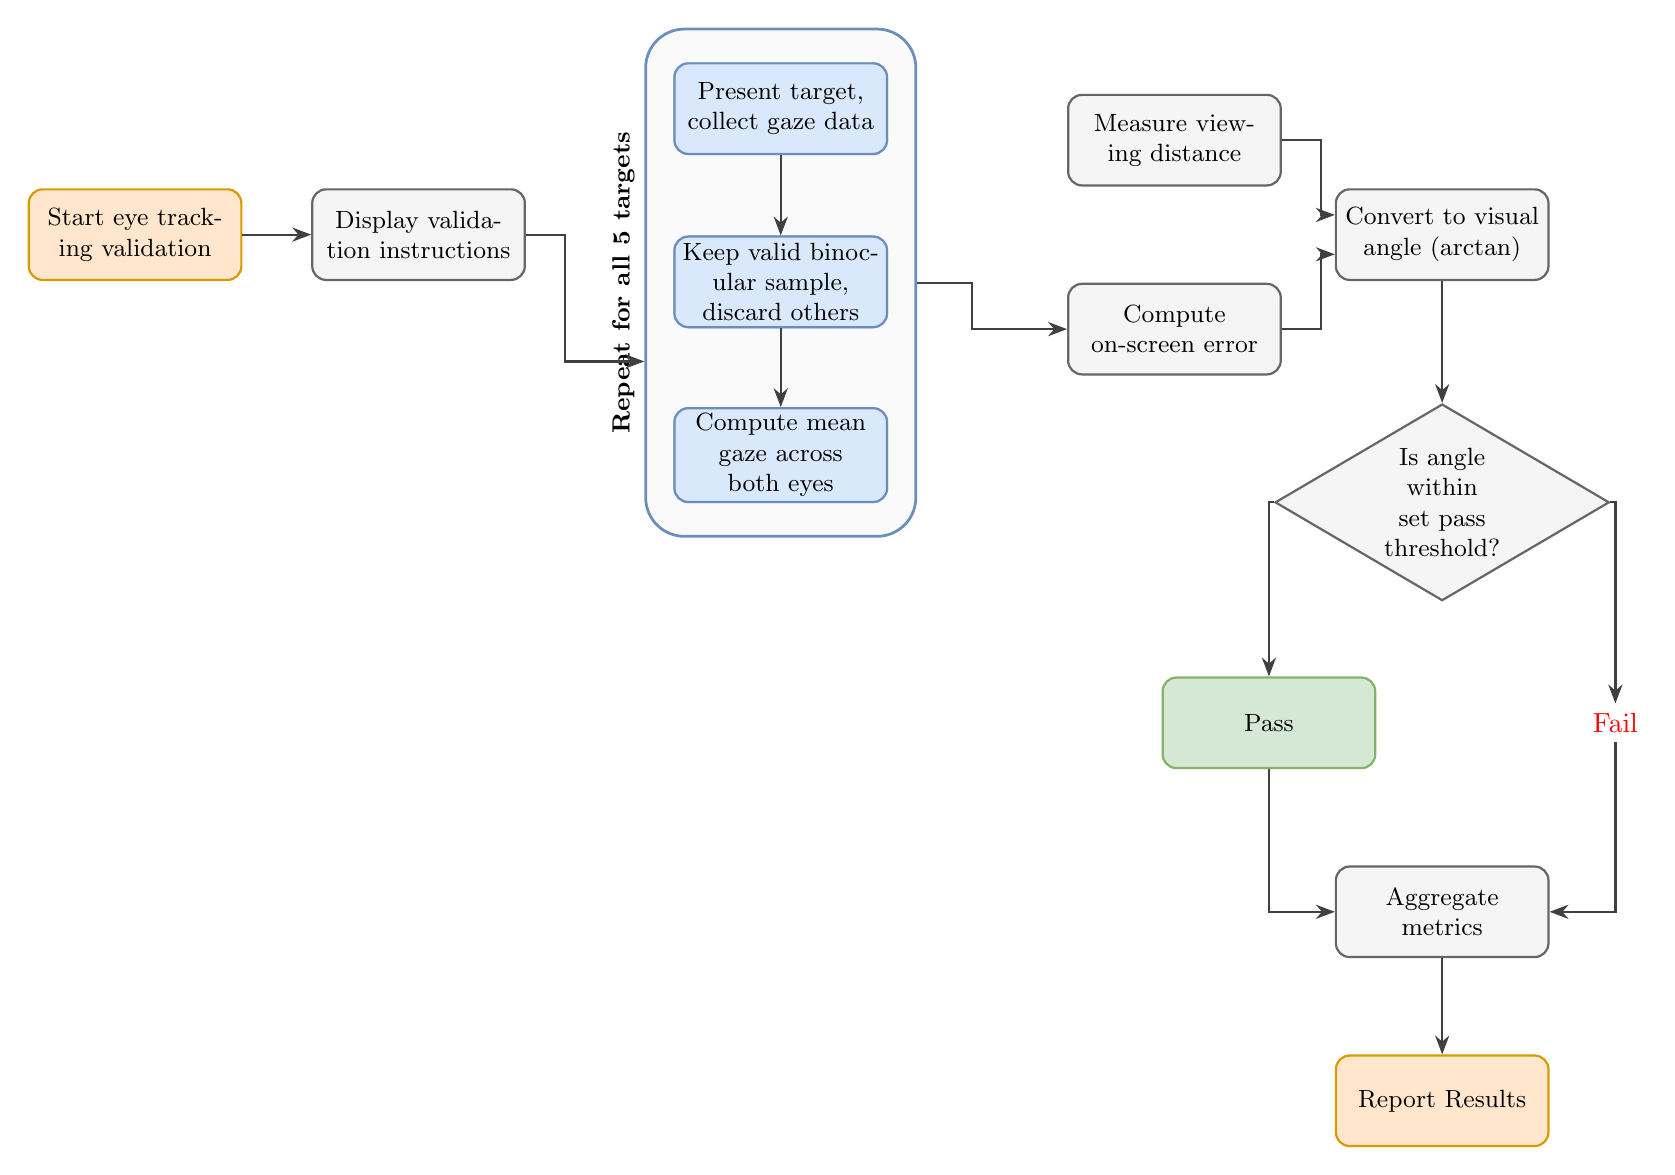
\begin{tikzpicture}

  % ---- Entry -------------------------------------------------------------
  \node[orange] (start) at (0,0)    {Start eye tracking validation};
  \node[gray]   (instr) at (3.6,0)  {Display validation instructions};

  % ---- Repeat-for-all-5-targets container --------------------------------
  \node[blue]   (present) at (8.2,1.6)  {Present target, collect gaze data};
  \node[blue]   (keep)    at (8.2,-0.6) {Keep valid binocular sample, discard others};
  \node[blue]   (mean)    at (8.2,-2.8) {Compute mean gaze across both eyes};

  \node[draw=dioBlueS, line width=1pt, fill=dioGrayF, fill opacity=0.45,
        rounded corners=14pt, inner xsep=10pt, inner ysep=12pt,
        fit=(present)(keep)(mean)] (loop) {};
  % redraw the inner nodes above the translucent container fill
  \node[blue] at (8.2,1.6)  {Present target, collect gaze data};
  \node[blue] at (8.2,-0.6) {Keep valid binocular sample, discard others};
  \node[blue] at (8.2,-2.8) {Compute mean gaze across both eyes};
  \node[rotate=90, font=\small\bfseries, anchor=south]
        at (loop.west) {Repeat for all 5 targets};

  \draw[flow] (present) -- (keep);
  \draw[flow] (keep) -- (mean);

  % ---- Post-loop metric computation --------------------------------------
  \node[gray] (dist)  at (13.2,1.2)  {Measure viewing distance};
  \node[gray] (err)   at (13.2,-1.2) {Compute on-screen error};
  \node[gray] (angle) at (16.6,0)    {Convert to visual angle (arctan)};

  \draw[flow] (instr.east) -- ++(0.5,0) |- ($(loop.west)+(0,-1)$);
  \draw[flow] (loop.east) -- ++(0.7,0) |- (err.west);
  \draw[flow] (dist.east) -- ++(0.5,0) |- ($(angle.west)+(0,0.25)$);
  \draw[flow] (err.east)  -- ++(0.5,0) |- ($(angle.west)+(0,-0.25)$);

  % ---- Threshold decision and outcomes ------------------------------------
  \node[decision] (thresh) at (16.6,-3.4) {Is angle within set pass threshold?};
  \node[green] (pass) at (14.4,-6.2) {Pass};
  \node[red]   (fail) at (18.8,-6.2) {Fail};
  \node[gray]  (agg)  at (16.6,-8.6) {Aggregate metrics};
  \node[orange](rep)  at (16.6,-11)  {Report Results};

  \draw[flow] (angle) -- (thresh);
  \draw[flow] (thresh.west) -| (pass.north);
  \draw[flow] (thresh.east) -| (fail.north);
  \draw[flow] (pass.south) |- ($(agg.west)+(-0.4,0)$) -- (agg.west);
  \draw[flow] (fail.south) |- ($(agg.east)+(0.4,0)$) -- (agg.east);
  \draw[flow] (agg) -- (rep);

  \draw[flow] (start) -- (instr);

\end{tikzpicture}
\end{document}
